\documentclass[10pt]{article}
\usepackage[paperwidth=11.8cm,paperheight=4.5cm,margin=0pt]{geometry}
\usepackage{tikz}
\usepackage{amsmath,amssymb}
\usepackage{mathptmx}
\pagestyle{empty}
\begin{document}
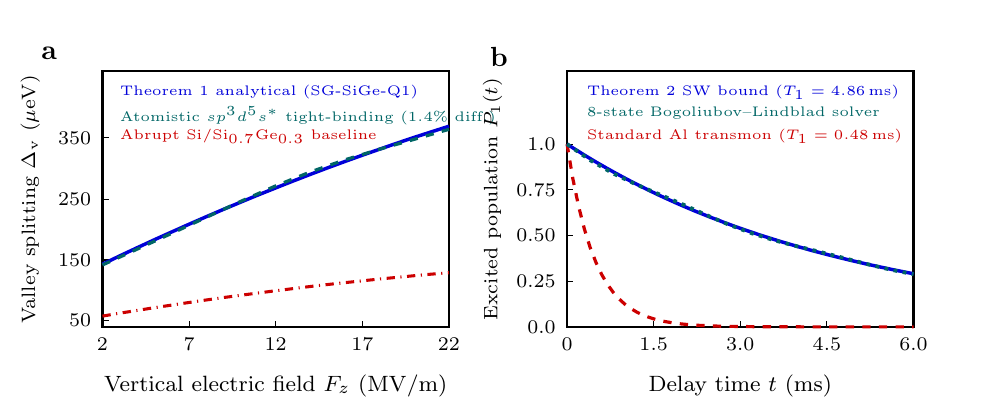
\begin{tikzpicture}[x=1cm,y=1cm]
  \useasboundingbox (0,0) rectangle (11.8,4.5);

  % Panel a: Tight-Binding vs Analytical Envelope Stark Tuning
  \node[anchor=north west,font=\bfseries\normalsize] at (0.05,4.38) {a};
  \draw[thick] (0.95,0.70) rectangle (5.35,3.95);
  \foreach \v/\y in {50/0.78, 150/1.55, 250/2.32, 350/3.10} {
    \draw (0.95,\y) -- (1.03,\y);
    \node[left,font=\scriptsize] at (0.93,\y) {\v};
  }
  \foreach \xval/\xpos in {2/0.95, 7/2.05, 12/3.15, 17/4.25, 22/5.35} {
    \draw (\xpos,0.70) -- (\xpos,0.78);
    \node[below,font=\scriptsize] at (\xpos,0.68) {\xval};
  }
  \node[below,font=\footnotesize] at (3.15,0.22) {Vertical electric field $F_z$ ($\mathrm{MV/m}$)};
  \node[rotate=90,above,font=\scriptsize] at (0.28,2.32) {Valley splitting $\Delta_{\mathrm{v}}$ ($\mu\mathrm{eV}$)};

  \draw[blue!85!black,line width=1.25pt] (0.950,1.496) -- (1.170,1.602) -- (1.390,1.705) -- (1.610,1.807) -- (1.830,1.906) -- (2.050,2.004) -- (2.270,2.100) -- (2.490,2.194) -- (2.710,2.286) -- (2.930,2.377) -- (3.150,2.465) -- (3.370,2.552) -- (3.590,2.637) -- (3.810,2.720) -- (4.030,2.801) -- (4.250,2.880) -- (4.470,2.957) -- (4.690,3.033) -- (4.910,3.107) -- (5.130,3.178) -- (5.350,3.248);
  \draw[teal!80!black,dashed,line width=1.15pt] (0.950,1.486) -- (1.390,1.687) -- (1.830,1.888) -- (2.270,2.092) -- (2.710,2.296) -- (3.150,2.491) -- (3.590,2.668) -- (4.030,2.822) -- (4.470,2.957) -- (4.910,3.082) -- (5.350,3.209);
  \draw[red!80!black,dashdotted,line width=1.1pt] (0.950,0.837) -- (1.170,0.874) -- (1.390,0.909) -- (1.610,0.944) -- (1.830,0.977) -- (2.050,1.010) -- (2.270,1.042) -- (2.490,1.073) -- (2.710,1.102) -- (2.930,1.131) -- (3.150,1.159) -- (3.370,1.186) -- (3.590,1.213) -- (3.810,1.238) -- (4.030,1.262) -- (4.250,1.285) -- (4.470,1.308) -- (4.690,1.329) -- (4.910,1.350) -- (5.130,1.370) -- (5.350,1.388);

  \node[anchor=north west,font=\tiny,blue!85!black] at (1.05,3.90) {Theorem 1 analytical (SG-SiGe-Q1)};
  \node[anchor=north west,font=\tiny,teal!80!black] at (1.05,3.62) {Atomistic $sp^3d^5s^*$ tight-binding ($1.4\%$ diff.)};
  \node[anchor=north west,font=\tiny,red!80!black] at (1.05,3.34) {Abrupt $\mathrm{Si/Si_{0.7}Ge_{0.3}}$ baseline};

  % Panel b: 8-State Bogoliubov-Lindblad vs Schrieffer-Wolff T1 Decay
  \node[anchor=north west,font=\bfseries\normalsize] at (5.75,4.38) {b};
  \draw[thick] (6.85,0.70) rectangle (11.25,3.95);
  \foreach \v/\y in {0.0/0.70, 0.25/1.28, 0.50/1.86, 0.75/2.44, 1.0/3.02} {
    \draw (6.85,\y) -- (6.93,\y);
    \node[left,font=\scriptsize] at (6.83,\y) {\v};
  }
  \foreach \xval/\xpos in {0/6.85, 1.5/7.95, 3.0/9.05, 4.5/10.15, 6.0/11.25} {
    \draw (\xpos,0.70) -- (\xpos,0.78);
    \node[below,font=\scriptsize] at (\xpos,0.68) {\xval};
  }
  \node[below,font=\footnotesize] at (9.05,0.22) {Delay time $t$ ($\mathrm{ms}$)};
  \node[rotate=90,above,font=\scriptsize] at (6.15,2.32) {Excited population $P_1(t)$};

  \draw[red!80!black,dashed,line width=1.15pt] (6.850,3.021) -- (6.923,2.585) -- (6.997,2.230) -- (7.070,1.943) -- (7.143,1.709) -- (7.217,1.519) -- (7.290,1.365) -- (7.363,1.240) -- (7.437,1.138) -- (7.510,1.056) -- (7.583,0.989) -- (7.657,0.935) -- (7.730,0.891) -- (7.803,0.855) -- (7.877,0.826) -- (7.950,0.802) -- (8.023,0.783) -- (8.097,0.767) -- (8.170,0.755) -- (8.243,0.744) -- (8.317,0.736) -- (8.390,0.729) -- (8.463,0.724) -- (8.537,0.719) -- (8.610,0.716) -- (8.683,0.713) -- (8.757,0.710) -- (8.830,0.708) -- (8.903,0.707) -- (8.977,0.706) -- (9.050,0.704) -- (9.123,0.704) -- (9.197,0.703) -- (9.270,0.702) -- (9.343,0.702) -- (9.417,0.702) -- (9.490,0.701) -- (9.563,0.701) -- (9.637,0.701) -- (9.710,0.701) -- (9.783,0.701) -- (9.857,0.700) -- (9.930,0.700) -- (10.003,0.700) -- (10.077,0.700) -- (10.150,0.700) -- (10.223,0.700) -- (10.297,0.700) -- (10.370,0.700) -- (10.443,0.700) -- (10.517,0.700) -- (10.590,0.700) -- (10.663,0.700) -- (10.737,0.700) -- (10.810,0.700) -- (10.883,0.700) -- (10.957,0.700) -- (11.030,0.700) -- (11.103,0.700) -- (11.177,0.700) -- (11.250,0.700);
  \draw[blue!85!black,line width=1.25pt] (6.850,3.021) -- (6.923,2.974) -- (6.997,2.928) -- (7.070,2.882) -- (7.143,2.838) -- (7.217,2.794) -- (7.290,2.752) -- (7.363,2.710) -- (7.437,2.669) -- (7.510,2.629) -- (7.583,2.590) -- (7.657,2.551) -- (7.730,2.514) -- (7.803,2.477) -- (7.877,2.440) -- (7.950,2.405) -- (8.023,2.370) -- (8.097,2.336) -- (8.170,2.303) -- (8.243,2.270) -- (8.317,2.238) -- (8.390,2.207) -- (8.463,2.176) -- (8.537,2.146) -- (8.610,2.117) -- (8.683,2.088) -- (8.757,2.060) -- (8.830,2.032) -- (8.903,2.005) -- (8.977,1.978) -- (9.050,1.952) -- (9.123,1.927) -- (9.197,1.902) -- (9.270,1.877) -- (9.343,1.853) -- (9.417,1.830) -- (9.490,1.807) -- (9.563,1.784) -- (9.637,1.762) -- (9.710,1.741) -- (9.783,1.719) -- (9.857,1.699) -- (9.930,1.678) -- (10.003,1.658) -- (10.077,1.639) -- (10.150,1.620) -- (10.223,1.601) -- (10.297,1.583) -- (10.370,1.565) -- (10.443,1.547) -- (10.517,1.530) -- (10.590,1.513) -- (10.663,1.496) -- (10.737,1.480) -- (10.810,1.464) -- (10.883,1.449) -- (10.957,1.433) -- (11.030,1.418) -- (11.103,1.404) -- (11.177,1.389) -- (11.250,1.375);
  \draw[teal!80!black,dotted,line width=1.35pt] (6.850,3.021) -- (7.143,2.817) -- (7.437,2.647) -- (7.730,2.508) -- (8.023,2.383) -- (8.317,2.257) -- (8.610,2.125) -- (8.903,1.998) -- (9.197,1.888) -- (9.490,1.797) -- (9.783,1.721) -- (10.077,1.649) -- (10.370,1.574) -- (10.663,1.497) -- (10.957,1.427) -- (11.250,1.368);

  \node[anchor=north west,font=\tiny,blue!85!black] at (6.98,3.90) {Theorem 2 SW bound ($T_1=4.86\,\mathrm{ms}$)};
  \node[anchor=north west,font=\tiny,teal!80!black] at (6.98,3.62) {8-state Bogoliubov--Lindblad solver};
  \node[anchor=north west,font=\tiny,red!80!black] at (6.98,3.34) {Standard $\mathrm{Al}$ transmon ($T_1=0.48\,\mathrm{ms}$)};
\end{tikzpicture}
\end{document}
